\documentclass{article}

\usepackage{amsmath}
\usepackage{graphicx}

\begin{document}
\title{MCMD P3 -- Monte Carlo simulation of Compton scattering}
\author{Alex Arash Sand Kalaee\\ \texttt{kalaee@teorfys.lu.se}}
\maketitle
\section{First exercise}
We create a program that samples the photon path lengths according to the
exponential distribution in an environment defined by the attenuation
coefficient $\mu$ and the mass density of the material $\varrho$
\begin{equation}
p(d) \propto \exp\left[-\mu(h\nu)\varrho d\right]
\end{equation}
where the attenuation is dependent on the energy of the incoming photon.

The distribution for the obtained lengths at various energies are provided in
Fig~\ref{fig:1}.

\begin{figure}
\centering
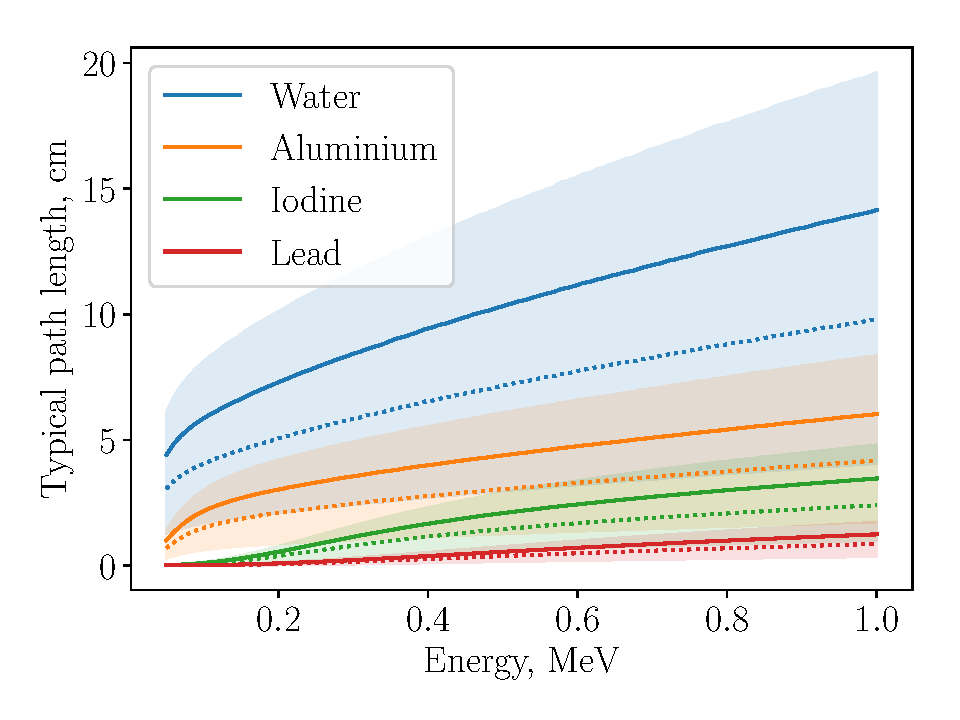
\includegraphics[width=0.8\textwidth]{first.pdf}
\caption{Characteristic path lengths  for the different materials:
water, aluminium, iodine and lead. The full line indicates the path mean,
the dotted the median and the shaded area are lengths in the
25\textsuperscript{th} to the 75\textsuperscript{th} percentile range.}
\label{fig:1}
\end{figure}

\section{Second exercise}
We construct a generator for Compton scattering of photons with input energy
$h\nu$ and output energy $h\nu'$ together with the corresponding scattering
angle $\theta$.
We plot the angular distribution as a function of energy in Fig~\ref{fig:2i}.
Next we determine the distribution of the energies of the scattered electrons,
see Fig~\ref{fig:2ii}. The electron energies are scaled according to the
incoming photon in order to have a similar region of comparison at all energies.
For the peak points in Fig~\ref{fig:2ii} we samples the corresponding angles
and find that the energy peaks at a scattering angle of $170^\circ$.

\begin{figure}
\centering
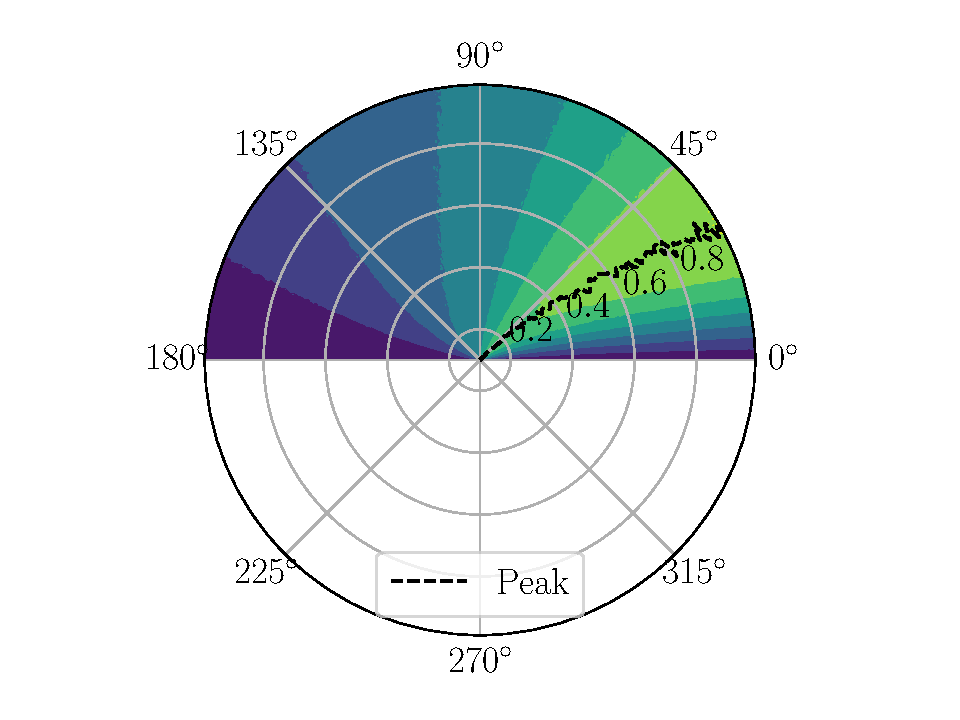
\includegraphics[width=0.8\textwidth]{secondi.pdf}
\caption{Angular distribution of the scattered photons with energies in the
range 0.1 to 1 MeV. The dashed line indicate the peak angle.}
\label{fig:2i}
\end{figure}

\begin{figure}
\centering
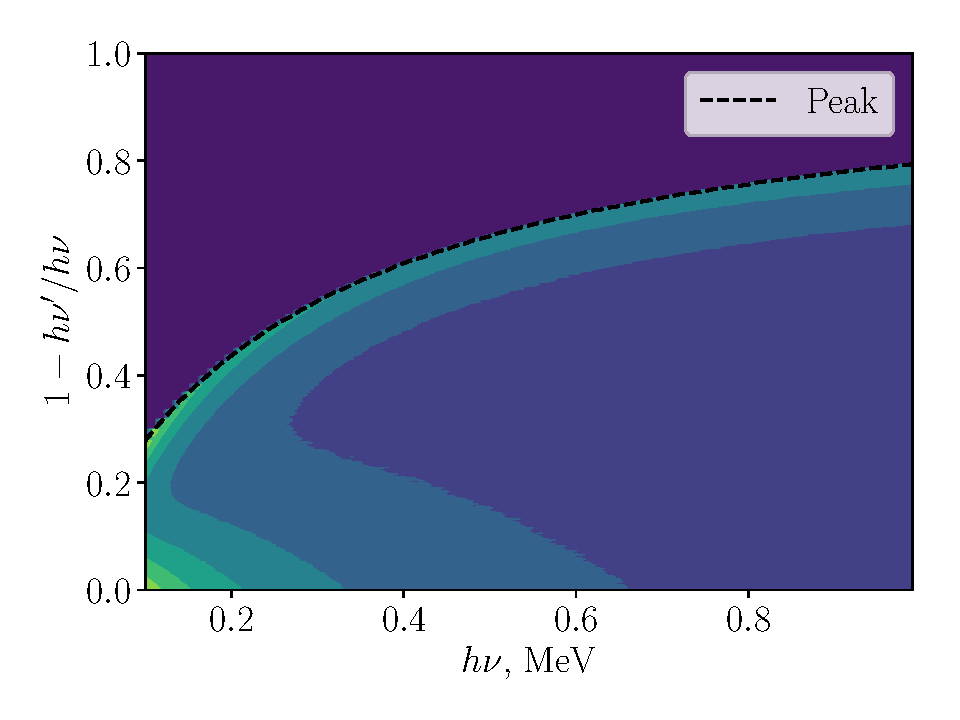
\includegraphics[width=0.8\textwidth]{secondii.pdf}
\caption{Distribution of energy of the scattered electrons relative to the
energy of the incoming photons. The dashed line indicates the peak.}
\label{fig:2ii}
\end{figure}

\end{document}
